\documentclass[11pt,a4paper]{article}
\usepackage[a4paper,margin=0.85in]{geometry}
\usepackage{amsmath,amssymb,booktabs,array}
\usepackage[T1]{fontenc}
\usepackage{lmodern}
\usepackage{xcolor}
\usepackage{hyperref}
\usepackage{listings}
\usepackage{graphicx}
\usepackage{enumitem}
\hypersetup{colorlinks=true,linkcolor=blue,urlcolor=blue,citecolor=blue}
\lstset{basicstyle=\ttfamily\small,breaklines=true,frame=single,backgroundcolor=\color{gray!8}}

\title{Intermediate Task 2 Report\\\large Goal-Conditioned Treasure Hunt using a Neural UVFA-Style Agent}
\author{AVD894 Reinforcement Learning Course Project}
\date{November 2026}

\begin{document}
\maketitle

\begin{abstract}
Intermediate Task 2 requires a complete simulator of the system being controlled
through reinforcement learning. We implement a goal-conditioned treasure-hunt
game and train a neural UVFA-style action-value model. The model receives both
the current state and a goal representation, and estimates the value of each of
four movement actions. Training uses online simulator experience, replay memory,
a target network, epsilon-greedy exploration, and a Huber temporal-difference
loss. The baseline run used 1,000 training episodes; a longer 5,000-episode run was
also measured. Both were evaluated on the same 500 held-out random episodes.
The longer run achieved a 100\% observed success rate and a mean successful
path length of 4.284 moves, close to the 4.280-move shortest-path reference.
\end{abstract}

\section{Idea: expected versus implemented}

The UVFA paper proposes a value function that is conditioned on both state and
goal. The expected behavior is that one learned model should be reusable for
different goals instead of requiring one independent policy per goal.

Our Task 2 implementation turns this idea into an interactive simulator. At the
start of an episode, the simulator samples a start cell and a different goal
cell from a fixed connected maze. The agent then chooses movement actions until
it reaches the goal or the maximum step limit is reached.

The implementation preserves the paper's central idea but is an explicit course
adaptation. The environment is a custom grid-based treasure hunt, and the model
uses an action-value head for direct control. We do not claim that the custom
maze or the measured numbers are the original paper's experimental results.

\section{Simulator and RL formulation}

The simulator contains an $8\times8$ maze with walls on the border and a small
number of internal obstacles. The observation is represented by:
\begin{itemize}[leftmargin=*]
    \item a one-hot encoding of the current agent cell plus the flattened obstacle map;
    \item a separate one-hot encoding of the goal cell.
\end{itemize}

For the current configuration, the state vector has dimension 128 and the goal
vector has dimension 64. The action space is
\[
\mathcal{A}=\{\text{up},\text{down},\text{left},\text{right}\}.
\]
An action into a wall leaves the agent in place. An episode terminates when the
agent reaches the goal and is truncated after 50 steps.

The base rewards are $+10$ for reaching the goal, $-0.1$ for a normal movement,
and $-1$ for a wall collision. To make the small simulator learnable within a
course-scale experiment, the current Task 2 configuration adds a documented
Manhattan-distance potential-shaping term:
\[
    r' = r + \lambda(d_{\text{old}}-d_{\text{new}}),
\]
where $\lambda=0.15$. This is an adaptation and is reported separately from
the paper's general UVFA idea. Task 1 uses the unshaped reward.

\section{Neural UVFA-style model}

The model has separate encoders for state and goal:
\[
    e_s=f_s(s;\theta_s), \qquad e_g=f_g(g;\theta_g).
\]
The two embeddings are concatenated and passed to an action-value head:
\[
    Q(s,g,\cdot;\theta)=h([e_s,e_g];\theta_h).
\]
The current network uses two fully connected hidden layers in each encoder and
an action-value head. Its dimensions are recorded in the checkpoint metadata:
hidden dimension 128 and embedding dimension 64.

Training is DQN-style. For a transition $(s,g,a,r,s',g',d)$, the target is
\[
    y=r+\gamma(1-d)\max_{a'}Q_{\mathrm{target}}(s',g',a';\theta^-),
\]
where $d$ indicates a terminal or truncated transition. The online network is
optimized with the Huber temporal-difference loss:
\[
    L(\theta)=\operatorname{Huber}
    \left(Q_{\mathrm{online}}(s,g,a;\theta),y\right).
\]
The replay buffer breaks temporal correlation, while the target network is
updated periodically to stabilize the target calculation.

\section{Training and testing procedure}

\subsection{Dataset and episode generation}

No external dataset was downloaded or used. This is a simulator-based control
problem. Training and testing episodes are generated online by the environment.
The fixed maze is specified in \texttt{configs/task2\_default.json}; start and
goal cells are sampled using controlled random seeds.

Training uses seed 2026. Episode $i$ uses the simulator seed $2026+i$. Testing
uses separate seeds $100000$ through $100499$. Both training budgets are
evaluated on the exact same held-out start/goal episodes to make the comparison
paired and reproducible.

\subsection{Training settings}

The baseline and extended runs used the same settings; only the number of
training episodes changed:
\begin{table}[h]
\centering
\caption{Task 2 training configuration.}
\begin{tabular}{ll}
\toprule
Setting & Value\\
\midrule
Training episodes & 1,000 baseline; 5,000 extended\\
Measured training wall time & about 53 seconds baseline; about 2.5 minutes extended\\
Maximum steps per episode & 50\\
Training seed & 2026\\
Discount factor & 0.95\\
Optimizer & Adam\\
Learning rate & 0.001\\
Replay capacity & 20,000 transitions\\
Batch size & 64\\
Replay warm-up & 200 transitions\\
Target update interval & 100 environment steps\\
Initial/final epsilon & 1.0 / 0.05\\
Epsilon decay steps & 5,000\\
Hidden dimension & 128\\
Embedding dimension & 64\\
Device & NVIDIA CUDA\\
PyTorch & 2.5.1+cu121\\
\bottomrule
\end{tabular}
\end{table}

In reinforcement learning, ``episodes'' are the primary training unit; this
experiment is not supervised learning with epochs over a fixed dataset. Every
episode produces new simulator transitions and the replay buffer is sampled for
updates during training.

\subsection{Commands and files}

The run can be reproduced from the project root with:
\begin{lstlisting}[language=bash]
python scripts/train_task2.py --config configs/task2_default.json \\
    --episodes 5000 --output artifacts/task2_extended_5000 --device auto

python scripts/evaluate_task2.py --config configs/task2_default.json \\
    --checkpoint artifacts/task2_extended_5000/checkpoint.pt \\
    --episodes 500 \\
    --output artifacts/task2_extended_5000/evaluation.json \\
    --device auto
\end{lstlisting}

The same workflow is available from
\texttt{notebooks/AVD894\_Task1\_Task2.ipynb}. The notebook displays the main
metrics and one learned rollout without requiring the user to type these
commands manually.

\section{Performance and results}

Each evaluation contains 500 held-out random episodes. Both learned checkpoints
were tested on the same seeds and compared with a breadth-first-search
shortest-path controller that knows the maze layout. The reference is a planning
baseline, not another learned policy. Success-rate intervals use the Wilson
95\% interval; path-length intervals use a percentile bootstrap with 20,000
resamples and seed 2026.

\begin{table}[ht]
\centering
\caption{Task 2 performance on the same 500 held-out episodes.}
\scriptsize
\begin{tabular}{p{0.30\linewidth}rrr}
\toprule
Metric & 1,000 episodes & 5,000 episodes & Shortest-path reference\\
\midrule
Success rate (95\% Wilson CI) & 98.6\% [97.14, 99.32] & 100.0\% [99.24, 100.00] & 100.0\%\\
Mean steps on successes (95\% bootstrap CI) & 4.546 [4.349, 4.744] & 4.284 [4.104, 4.466] & 4.280\\
Mean return & 9.901 & 10.138 & 10.138\\
\bottomrule
\end{tabular}
\end{table}

\begin{figure}[ht]
\centering
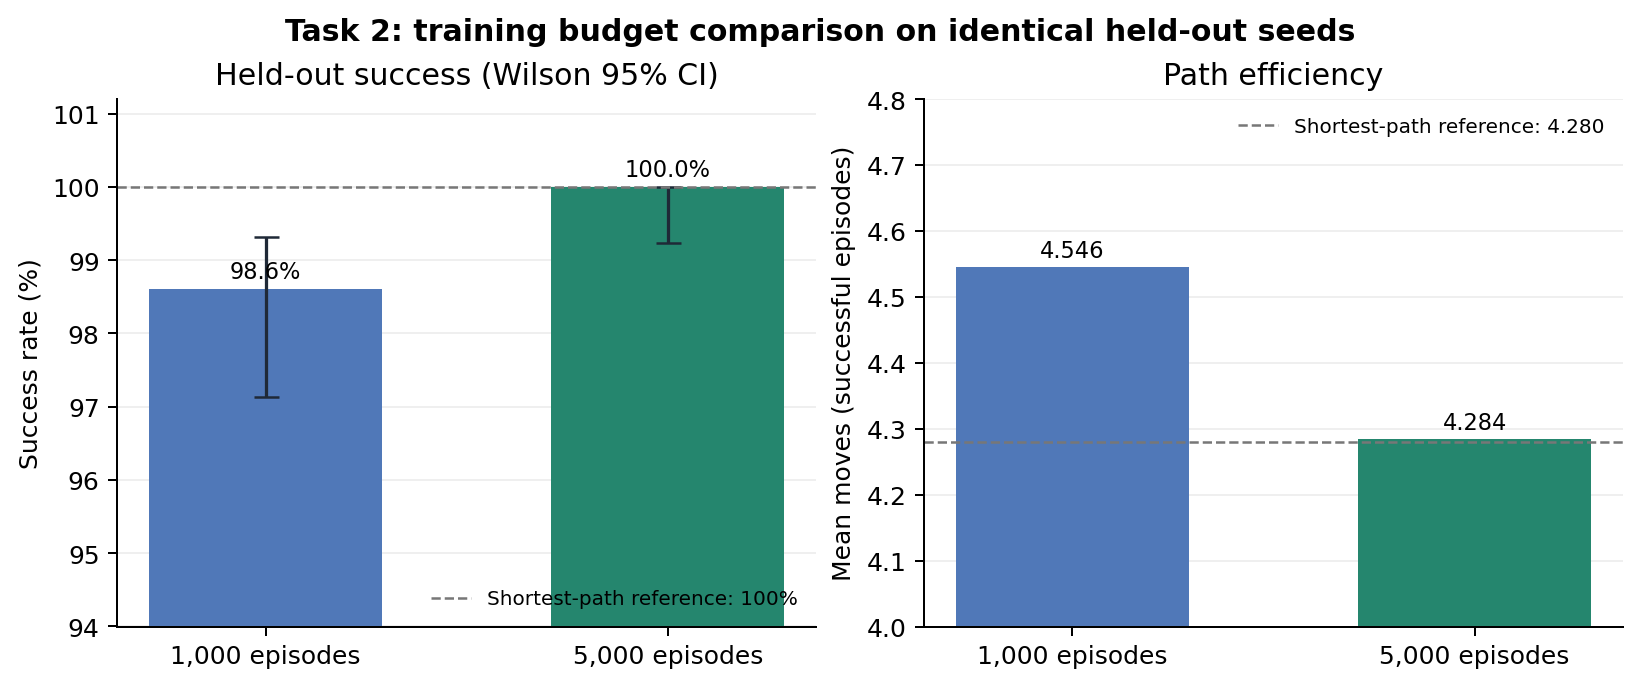
\includegraphics[width=0.96\linewidth]{task2_training_comparison.png}
\caption{Training-budget comparison on identical held-out episodes. Error bars in the success panel
show Wilson 95\% intervals. The 5,000-episode checkpoint reached all 500
goals and approached the shortest-path reference in moves.}
\label{fig:training-comparison}
\end{figure}

The 1,000-episode run missed 7 of 500 goals. The 5,000-episode run reached all
500 goals and lowered the mean successful path length to 4.284, within 0.004
moves of the shortest-path reference on this sample. The data support a
training-budget improvement on this fixed maze and seed set. They do not show
generalization to new maps, and the single training seed means run-to-run
variation has not been estimated. The 100\% observed rate is not a guarantee of
perfect future performance; its Wilson lower bound is 99.24\%.

The 5,000-episode evaluation is stored in
\texttt{artifacts/task2\_extended\_5000/evaluation.json}; its checkpoint and
episode-level training log are stored beside it. The baseline result remains in
\texttt{artifacts/task2\_submission\_1000/}.

\section{Demonstration output}

The project provides two demonstration modes:
\begin{enumerate}[leftmargin=*]
    \item The notebook displays an ASCII rollout and the aggregate evaluation metrics.
    \item \texttt{scripts/demo.py} opens a Tkinter window showing walls, the blue agent,
    the green goal, visited path, last action and reward, episode return, and step count.
    The interface supports single-step control and animated auto-play.
\end{enumerate}

The graphical interface is useful for presentation, while the JSON output is the
auditable source for reported metrics. A screenshot of the interface can be
added to the final presentation if required; it is not necessary for the
mathematical content of this report.

\section{Limitations and future work}

The current result is strong for the fixed small maze but should not be
overgeneralized. The model has not yet been tested on arbitrary obstacle maps,
larger grid sizes, or changing transition dynamics. The distance shaping term
also makes this an adaptation rather than a strict paper reproduction. Future
work can evaluate randomized maps, compare shaped and unshaped rewards, and
test generalization to larger mazes. Those experiments should be reported as
extensions and not mixed with the Task 2 baseline.

\section{References}

\begin{thebibliography}{9}
\bibitem{schaul2015}
Tom Schaul, Daniel Horgan, Karol Gregor, and David Silver,
``Universal Value Function Approximators,''
\emph{Proceedings of the 32nd International Conference on Machine Learning},
PMLR 37, pp. 1312--1320, 2015.
\url{https://proceedings.mlr.press/v37/schaul15.html}
\end{thebibliography}

\end{document}

